\chapter{Diffusion Maps}
\section{Introduction}

Diffusion Maps are a technique for discovering underlying geometricity of a graph $G=(V,E)$ solely from the connectivity. We will put the technique to use in order to invert the GIRG generative process - go from a graph produced by a $d$-dimensional GIRG, and infer the original locations $(x_u)_{u\in V}$ of the vertices $x_u \in \T^d$.

The idea of Diffusion Maps is to analyse the diffusion process of random walking on the edges of the graph, and to characterise the probability cloud starting from one node in the graph as a sum of decreasingly important contributions, along the line of eigenvectors of decreasing eigenvalues from a diagonalisable matrix. The top $d$ contributions can then be used as a coordinate system to describe each point in the graph. By taking a large timestep diffusion cloud, the general relative location of the initial point is the main signal. The hope is that if connections (probabilistically) follow a geometry of $d$-dimensions, then the diffusion map coordinate system will capture / align with this real geometry.

The diffusion process is defined by the transition matrix $M = D^{-1}W$, where $D$ is the diagonal matrix with $D_{uu} = \sum_{v\in V} W_{uv}$ is the diagonal degree matrix, and $W_{uv}$ is the adjacency matrix, $W_{uv} = \begin{cases}1 & u \sim v \\0 & u \nsim v \end{cases}$. The matrix $S = D^{-1/2} W D^{-1/2}$ is a symmetrised version and hence is diagonalisable as $S = V \Lambda V^T$. Then the map $M = D^{-1/2} S D^{1/2} = D^{-1/2} V \Lambda (D^{1/2} V)^T = \Phi \Lambda \Psi^T$.

In particular, starting at node $i$ (numbered $i=1,...,n$), the $t$th step diffusion cloud is $i \mapsto M^t_{ij} = (\Phi \Lambda^t \Psi^T)_{ij} = \sum_{k=1}^n \Phi_{ik} \lambda_k^t \Psi_{jk}$.

So writing $\Phi = [\phi_1, \phi_2, ..., \phi_n]$ and $\Psi = [\psi_1, \psi_2, ..., \psi_n]$, we have that the $t$th step diffusion cloud is $i \mapsto \sum_{k=1}^n \phi_k(i) \lambda_k^t \vec{\psi}_k$. I.e. the diffusion map coordinate system is $\text{diffmap}_t(i) = (\lambda_2^t \phi_2(i), \lambda_3^t \phi_3(i), ..., \lambda_{d+1}^t \phi_{d+1}(i))$. The first coordinate is always $1$, it's the stationary distribution that all diffusion clouds converge to, so is discarded.

\section{Diffusion Maps on GIRGs}
If we have a graph $G$ which we know is generated from a $d$-dimensional GIRG, we can simply extract the $d$-truncated diffusion map coordinates of each node as an estimate for the original geometric location of the node.

If $d$ is unknown, diffusion maps present one way to infer the dimensionality by analysing the ordered sequence of eigenvalues $\lambda_2 < \lambda_3 < ...$. In theory there is a good cutoff point whereby the first $d$ eigenvalues are of similar large size, and the rest are much smaller. This indeed works well for graphs synthetically generated from GIRGs, not so well on real world graphs.


We see in \cref{fig:cube_diffmap_plots_d2} that the inferred first two diffusion map coordinates do fit a square quite well. In general the points will be centered around the origin, as all $\lambda_2, \lambda_3, ...$ eigenvalue evectors will be orthogonal to the stationary distribution $\vec{\phi}_1 = k \vec{1}$ : they represent a deviation from the stationary distribution - e.g. for a node on the 1D line towards left end, it will need to put more diffusion probability on the left side nodes, and less on the right side nodes than the stationary distribution. The scale is quite tiny, as $\lambda_2 < 1$, and is decreasing with $t$. Furthermore for fixed $t$, the scale for $a < b$, the ath coordinate diffmap points will have larger scale than the bth coordinate as $\lambda_a > \lambda_b$.

The 0 centering can easily be fixed to be more Cube GIRG like by shifting the points $(\vec{x}_u)_i \gets (\vec{x}_u)_i + \min_v (\vec{x}_v)_i$.

The scaling can be see either as a bug or a feature. If we are certain that the points should be (relatively uniformly) distributed within the unit cube, then we can simply rescale separately along each dimension.
A linear coordinatewise scaling $x \gets \frac{x - x_{\min}}{x_{\max} - x_{\min}}$ works, or more extremely a coordinatewise "uniformify" procedure that replaces $(x_u)_i$ with its percentile value compared with other $(x_v)_i$.
In \cref{fig:diffmap_uniformed_vs_nonuniformed} we see uniformified versions of a generated 2D GIRG, and the socfb-Amherst41 graph.

Seen as a feature, the relatively different scaling allows as a natural correction to the potential non equivalence of different dimensions. For instance in a weighted euclidean norm setup, it could be that a 2D GIRG's true 1st geometric dimension (between $[0, 1]$) is much more important than its 2nd geometric dimension in determining the distance: $\norm{x - y} = \sqrt{a (x_1 - y_1)^2 + b(x_2 - y_2)^2}$. In this case, the diffusion map coordinates will have a larger scale for the $\lambda_2$ coordinate than the $\lambda_3$ coordinate, and the points will look like an elongated rectangle. The flatness of $\lambda_2, \lambda_3, \lambda_4, \lambda_5$ line segment in \cref{fig:cube_diffmaps_d4} is a testament to the cube (and non cuboidness) of the underlying GIRG that generated the graph. 


% TODO put in some eigenvalue plots

\begin{figure}
    \centering

    \begin{subfigure}{0.45\textwidth}
      \centering
      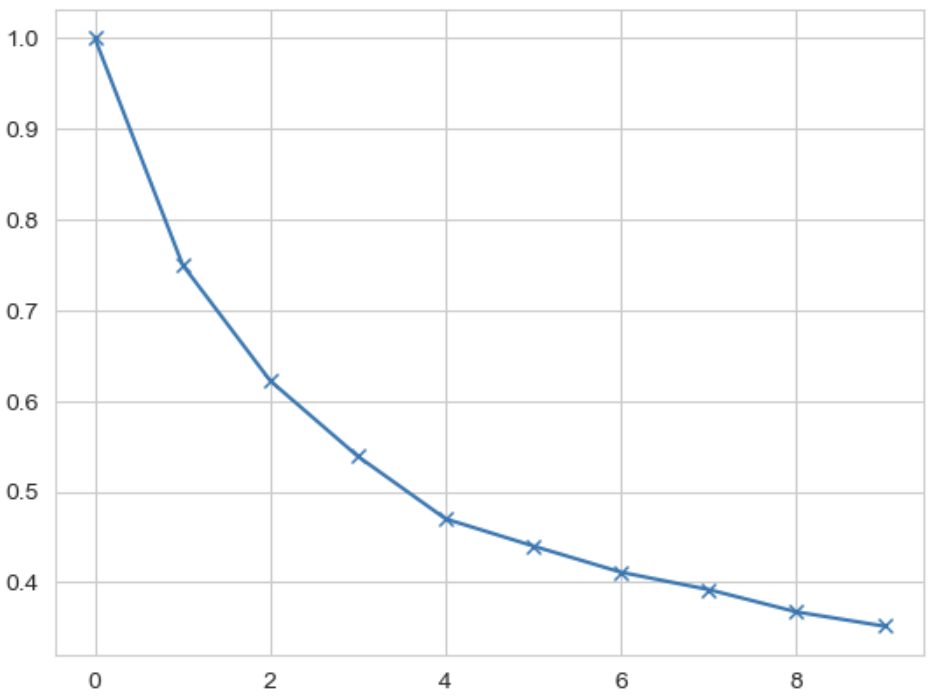
\includegraphics[width=\linewidth]{figures/diffmap_1d.png}
      \caption{$d=1$}
    \end{subfigure}
    \hfill
    \begin{subfigure}{0.45\textwidth}
      \centering
      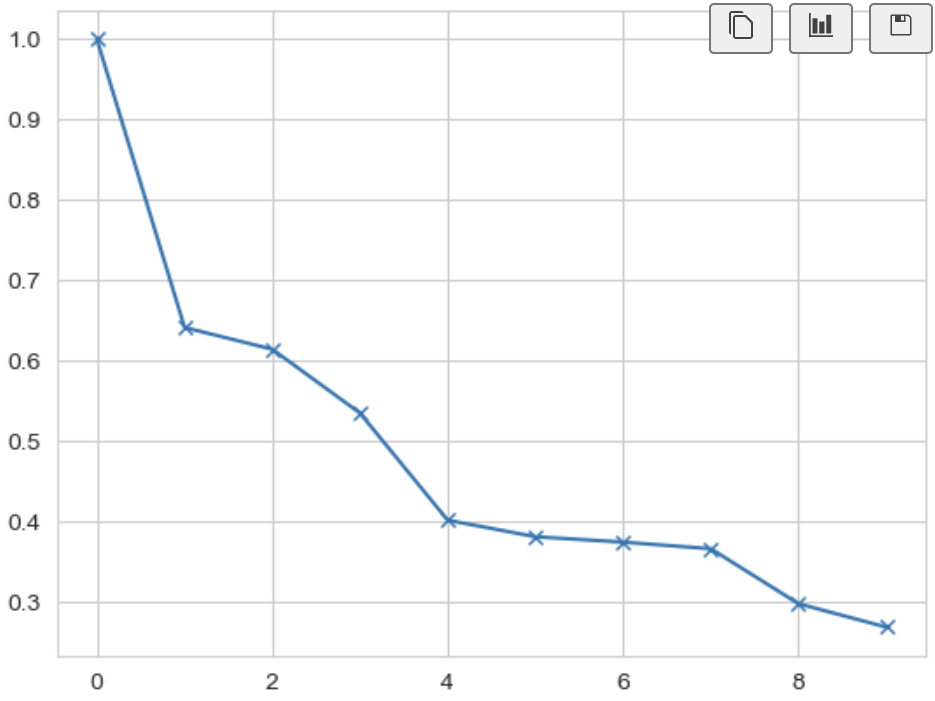
\includegraphics[width=\linewidth]{figures/diffmap_2d.png}
      \caption{$d=2$}
    \end{subfigure}
  
    \vspace{1em}
  
    \begin{subfigure}{0.45\textwidth}
      \centering
      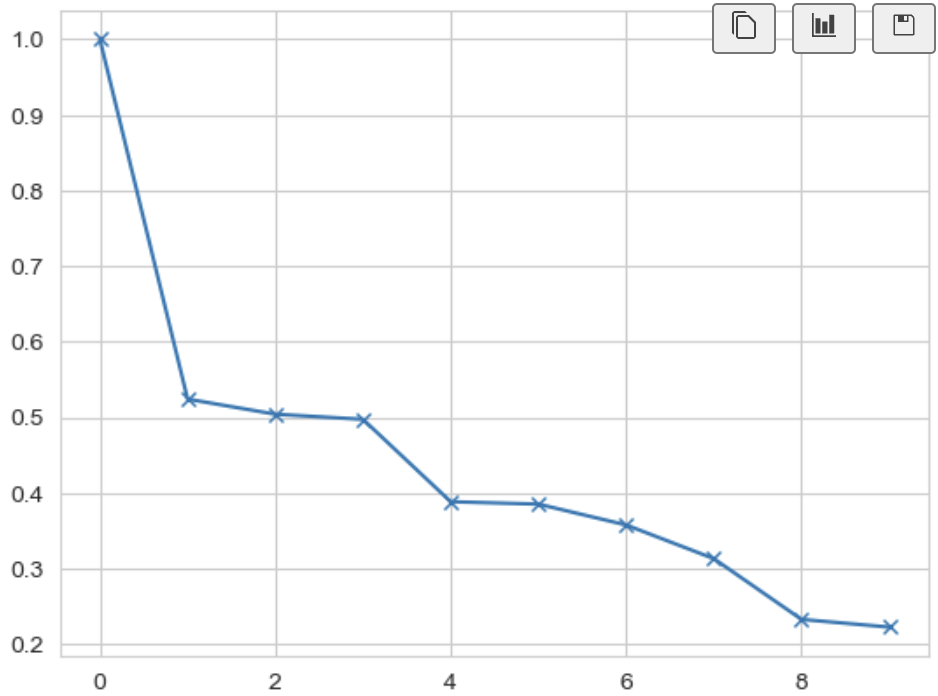
\includegraphics[width=\linewidth]{figures/diffmap_3d.png}
      \caption{$d=3$}
    \end{subfigure}
    \hfill
    \begin{subfigure}{0.45\textwidth}
      \centering
      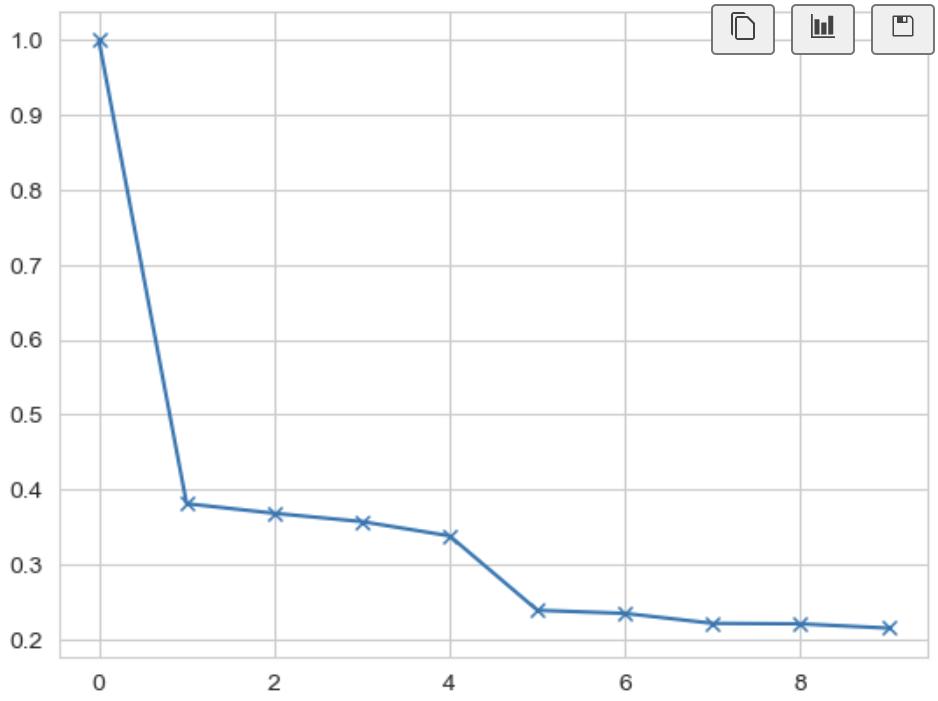
\includegraphics[width=\linewidth]{figures/diffmap_4d.png}
      \caption{$d=4$}
      \label{fig:cube_diffmaps_d4}
    \end{subfigure}
  
    \caption{Diffusion map eigenvalues (including $\lambda_1 = 1$) for a $n=2000, \tau=2.5, \alpha=1.3$ Cube GIRG with $d=1,2,3,4$ dimensions.}
    \label{fig:cube_diffmaps_d1to4}
\end{figure}

\begin{figure}
    \centering

    \begin{subfigure}{0.45\textwidth}
      \centering
      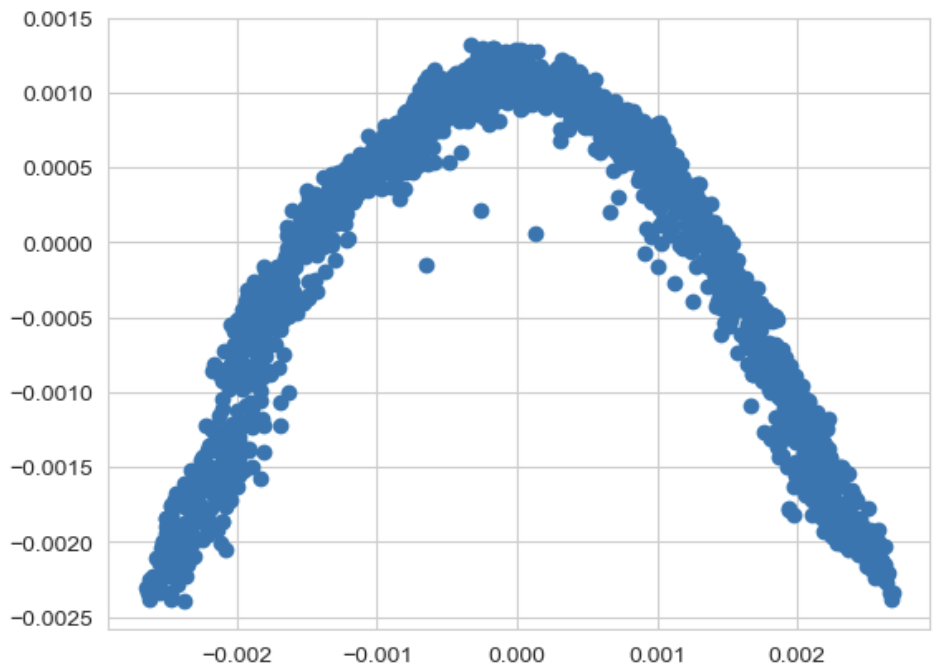
\includegraphics[width=\linewidth]{figures/diffmap_1d_plot.png}
      \caption{$d=1$}
      \label{fig:sub1}
    \end{subfigure}
    \hfill
    \begin{subfigure}{0.45\textwidth}
      \centering
      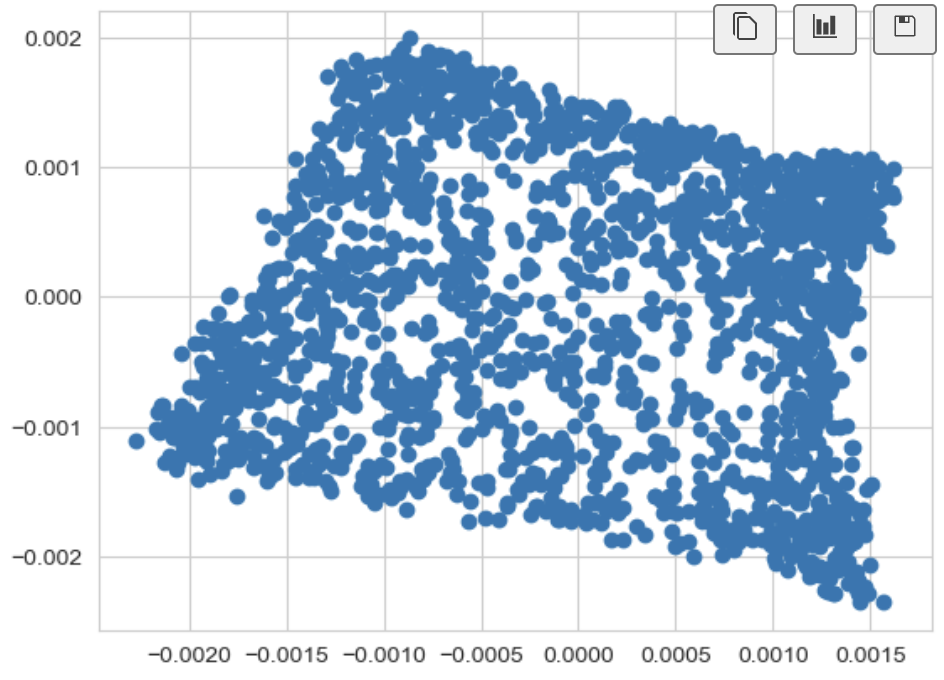
\includegraphics[width=\linewidth]{figures/diffmap_2d_plot.png}
      \caption{$d=2$}
      \label{fig:cube_diffmap_plots_d2}
    \end{subfigure}

  
    \caption{Diffusion map scatter plot of the first two extracted coordinates from 1d and 2d GIRGs.}
    \label{fig:cube_diffmap_plots_d1and2}
\end{figure}


\begin{figure}
    \centering

    \begin{subfigure}{0.45\textwidth}
      \centering
      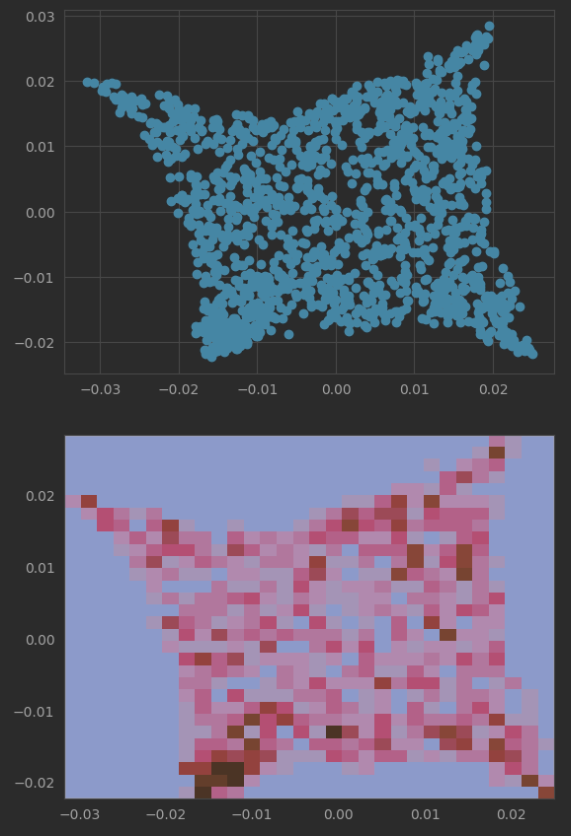
\includegraphics[width=\linewidth]{figures/diffmap_plot_nonuniformed.png}
      \caption{2d GIRG non-uniformed}
      \label{fig:sub1}
    \end{subfigure}
    \hfill
    \begin{subfigure}{0.45\textwidth}
      \centering
      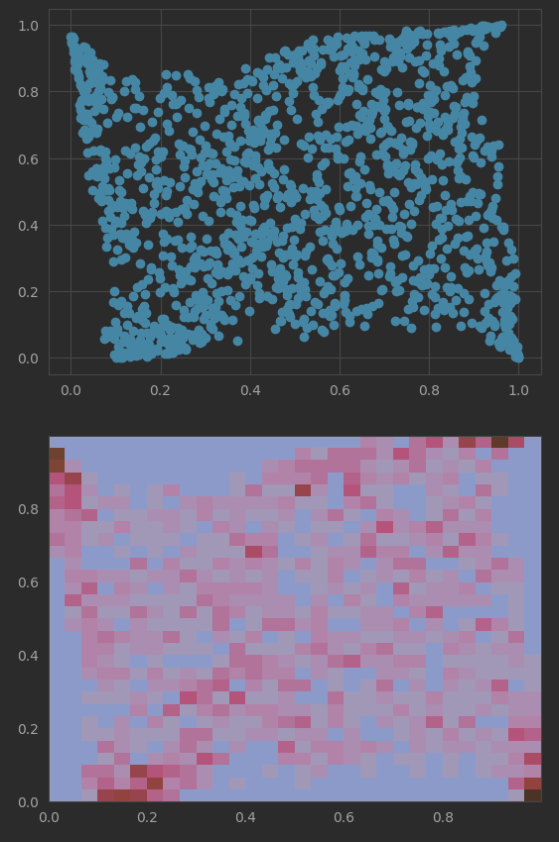
\includegraphics[width=\linewidth]{figures/diffmap_plot_uniformed.png}
      \caption{2d GIRG uniformed}
      \label{fig:sub2}
    \end{subfigure}
  
    \vspace{1em}
  
    \begin{subfigure}{0.45\textwidth}
      \centering
      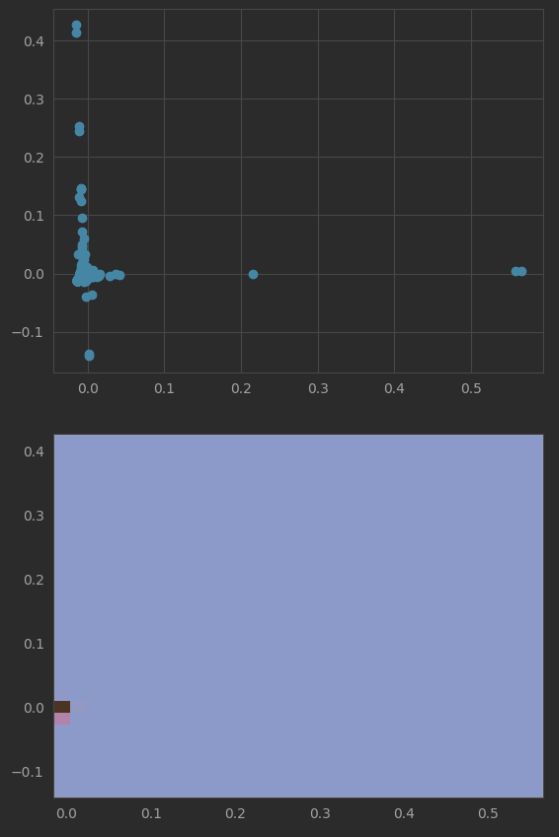
\includegraphics[width=\linewidth]{figures/real_diffmap_plot_nonuniformed.png}
      \caption{socfb-Amherst41 non-uniformed}
      \label{fig:sub3}
    \end{subfigure}
    \hfill
    \begin{subfigure}{0.45\textwidth}
      \centering
      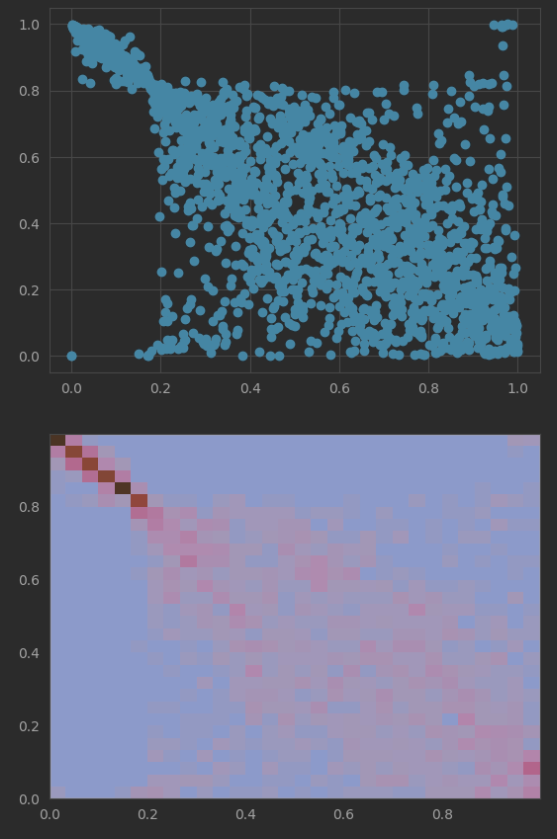
\includegraphics[width=\linewidth]{figures/real_diffmap_plot_uniformed.png}
      \caption{socfb-Amherst41 uniformed}
      \label{fig:sub4}
    \end{subfigure}
  
    \caption{Diffusion map scatter plot of the first two extracted coordinates, with and without using an additional uniform square remapping}
    \label{fig:diffmap_uniformed_vs_nonuniformed}
\end{figure}



Interestingly Toroidal GIRGs are differentiated from Cube GIRGs in that the diffusion map requires $2d$ coordinates to capture the Torus geometry instead of just $d$ for the cube.


One issue with diffusion maps is that even if the graph was Cube GIRG generated, the diffusion map coordinates may be a (slightly malformed) rotation of the actual cube. The diffusion map also seems slightly over concentrated in its corners/edges. 


TODO 

- fuller analysis of different diffmap modes: 'uniformify', 'cubify' and 'cuboidify', comparing performance on real life and synthetic graphs

- presentation of the small degree stochastic walk tweak which improves diffusion map performance:
\begin{verbatim}
# Empirically this gamma seems to work well. 
# It discourages taking edges to popular nhbs.
gamma = 0.9
M_tilde = scipy.sparse.diags(1 / D) @ A @ scipy.sparse.diags(D ** (-gamma))
M_tilde = scipy.sparse.diags(np.array(1 / M_tilde.sum(axis=-1)).squeeze()) @ M_tild
\end{verbatim}

- is it true that diffusion map tends to cluster representations edges rather than being more uniform? Empricially seems to happen in 2D but not 1D?

